\documentclass[12pt,a4paper]{report}

%
% PACKAGES AND STYLES
%

% 
% Language and encoding
%
%\usepackage{mathtext}
%\usepackage[T2A]{fontenc}
\usepackage[utf8]{inputenc}
\usepackage[english,russian]{babel}
\usepackage{mmap}

%
% Colors
%
\usepackage[usenames]{color}
\usepackage{color}
\usepackage{colortbl}

%
% Symbols
%
\usepackage{amssymb}
\usepackage{MnSymbol}

%
% Units
%
%\usepackage[binary-units=true]{siunitx}
\newcommand{\km}{\mathrm{~\text{км}}}
\newcommand{\m}{\mathrm{~\text{м}}}
\newcommand{\s}{\mathrm{~\text{с}}}
\newcommand{\mps}{\m \s ^{-1}}
\newcommand{\pers}{\s ^{-1}}
\newcommand{\K}{\mathrm{~\text{К}}}
\newcommand{\Kpkm}{\K\km ^{-1}}
\newcommand{\hpa}{\mathrm{~\text{гПа}}}
\newcommand{\J}{\mathrm{~\text{Дж}}}
\newcommand{\Jpm}{\J \m ^{-3}}

%
% Paper size and margins
%
\usepackage{vmargin}
\setmarginsrb{2.5cm}{1cm}{2.5cm}{2cm}{0cm}{0cm}{0cm}{1.5cm}

%
% Page style
%
\usepackage{fancyhdr}
\setlength{\headheight}{16pt}
\newcommand{\changefont}{%
    \fontsize{9}{11}\selectfont
}
\fancyhf{}
\fancyhead[RO]{\changefont \slshape \rightmark} %section
\fancyhead[LO]{\changefont \slshape \leftmark} %chapter
\fancyfoot[C]{\changefont \thepage} %footer
\setlength{\headsep}{0.2in}
\pagestyle{fancy}

%
% Indenting
%
\usepackage{indentfirst}
\setlength{\parindent}{1cm}
\setlength{\parskip}{0.5cm}

%
% References
%
\usepackage{natbib}

%
% Hyperlinks
%
\usepackage[linktocpage=true,plainpages=false,pdfpagelabels=false]{hyperref}
\definecolor{linkcolor}{rgb}{0.1,0,0.9}
\definecolor{citecolor}{rgb}{0,0,0.9}
\definecolor{urlcolor}{rgb}{0,0,1}
\hypersetup{
    colorlinks, linkcolor={linkcolor},
    citecolor={citecolor}, urlcolor={urlcolor}
}

\bibliographystyle{plainnat}
% Bibliography: set article volume number in bold font
%\DeclareFieldFormat
%  [article]
%  {volume}{\textbf{#1}}
%\renewcommand\nameyeardelim{, }

%\usepackage{showkeys} % show labels

\newcommand{\figref}[1]{\mbox{Figure~\ref{#1}}}
\newcommand{\tabref}[1]{\mbox{Table~\ref{#1}}}
\newcommand{\secref}[1]{\mbox{Section~\ref{#1}}}
\newcommand{\chpref}[1]{\mbox{Chapter~\ref{#1}}}
\newcommand{\appref}[1]{\mbox{Appendix~\ref{#1}}}
\newcommand{\eqnref}[1]{\mbox{Eq.~(\ref{#1})}}
\newcommand{\listref}[1]{\mbox{Listing~(\ref{#1})}}

%
% Lists
%
\usepackage[shortlabels]{enumitem}

\newenvironment{sqlist}[1][\enskip$\filledsquare$]
        {\begin{itemize}[#1]}
        {\end{itemize}}

% New math commands
% differential d, from http://tex.stackexchange.com/a/60546/586
\newcommand*\diff{\mathop{}\!\mathrm{d}}
\newcommand\mean[1]{\overline{#1}}
\newcommand{\PDt}[2]{\partial #1/\partial #2}

%
% Tables
%
\usepackage{booktabs}
%\usepackage{tabularx}
\usepackage{tabu}
\usepackage{longtable}

%
% Figures
%
\usepackage{wrapfig}
\usepackage[font=small,textfont=it,labelfont=bf]{caption}
%\captionsetup[figure]{labelfont=bf}
\usepackage{tikz}
\usepackage{pgfplots}
\usetikzlibrary{calc}

%
% Equations
%
\usepackage{cool}


\begin{document}
\setcounter{chapter}{1}
\chapter{Механизмы генерации полярных мезоциклонов}
Исследование структуры и динамики мезомасштабных вихрей высоких широт породило множество теорий их возникновения \citep{RT2003}. Схожесть изображений полярных мезоциклонов и тропических ураганов на спутниковых снимках дала повод считать, что в основе эволюции полярных вихрей также лежит конвекция. Однако благодаря накопленным натурным данным и результатам моделирования в конце XX века стала общепринятой точка зрения, согласно которой существует спектр полярных мезомасштабных вихрей. В одной части этого спектра находятся мезоциклоны, которые на снимках из космоса выглядят как спиралевидные системы облачности и в образовании которых преимущество имеют конвективные процессы. На другом конце спектра --- чисто бароклинные образования в виде облачных запятых, механизм образования которых аналогичен механизму внетропических циклонов синоптического масштаба.

Выдвижение единой теории, строго определяющей развитие мезоциклона, обычно не было успешным, так как мезоциклоны чаще всего возникают как гибридные образования. На разных этапах их развития преобладает тот или иной фактор.

Одним из кандидатов на роль механизма развития мезоциклона являются диабатические процессы, связанные, например, с выделением скрытого тепла кондесации, а также потоков тепла с поверхности. С 1970-х гг. значительный вес имеет концепция условной неустойчивости второго рода (conditional instability of second kind, CISK). Идея CISK заключается во взаимодействии мезомасштабных горизонтальных и вторичных вертикальных движений, приводящем к постепенному высвобождению энергии неустойчивости внешней среды. В конце 1980-х внимание исследователей переключилось на теорию неустойчивости взаимодействия атмосферы и океана (air-sea interaction instability, ASII), позднее обозначаемую термином WISHE (wind-induced surface heat exchange), предложенную в работе \citep{EmanuelRotunno1989}. Согласно этой теории, ключевую роль в усилении мезоциклона, то есть в падении давления в центре, играют запасы тепла у поверхности.

В то время как значительная часть исследований посвящена конвективным механизмам, не нужно преуменьшать важность бароклинных процессов. Этот подход основан на понятии бароклинной неустойчивости, возникающей вследствие температурного градиента между воздухом над относительно теплой поверхностью воды и воздухом над относительно холодной поверхностью, например, морским льдом. Авторы одной из пионерных работ, посвященных полярным мезоциклонам, рассматривают мезоциклоны именно как бароклинные возмущения \citep{HarroldBrowning1969}. В подтверждение приводятся данные наблюдений, свидетельствовавшие о том, что полярная депрессия имела в себе восходящую и нисходящую воздушную массу, повторяя структуру внетропических циклонов умеренных широт. Добавим, что полярные мезоциклоны бароклинного типа обычно разделяют на категории в зависимости от географического района происхождения. Так, например, полярные депрессии с обратным сдвигом впервые были обнаружены в регионе северо-западной Атлантики, где они чаще всего и встречаются.

Таковы основные механизмы образования полярных мезомасштабных циклонических вихрей. Что же их объединяет? Каждый из этих процессов можно рассмотреть с точки зрения генерации кинетической энергии атмосферных движений и ее источника в виде доступной потенциальной энергии (ДПЭ), которая по-своему накапливается в том или ином процессе.

\section{Бароклинная неустойчивость}
Как известно, волновую неустойчивость атмосферы можно разделить на два типа: баротропную --- связанную с горизонтальным сдвигом ветра --- и бароклинную, которая связана со сдвигом ветра по высоте. Бароклинная неустойчивость атмосферы возникает при условии бароклинности атмосферы, что означает зависимость плотности воздуха не только от давления, но и от температуры. Другими словами, температура не постоянна на изобарической поверхности.

\begin{figure}
  \centering
  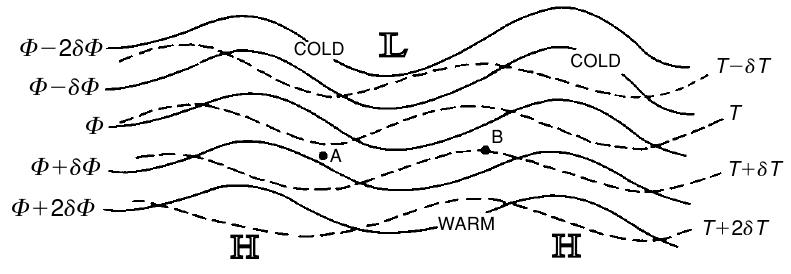
\includegraphics[width=\linewidth]{{./chapters/figures_misc/baroclinic_rt2003}.jpeg}
  \caption{Распределение изогипс (сплошные линии) и изотерм (пунктирные линии) на изобарической поверхности в развивающейся бароклинной волне в Северном полушарии \citep{RT2003}.}
  \label{fig:baroclinic_rt2003}
\end{figure}

В атмосфере средний поток, связанный с горизонтальным температурным градиентом на изобарических поверхностях, обладает доступной потенциальной энергией, которая может быть трансформирована в кинетическую, что вызовет спонтанный рост малых возмущений.

Принцип развития бароклинной волны в регионе с сильным температурным градиентом может быть объяснен следующим образом (рис. \ref{fig:baroclinic_rt2003}). Пусть в изначально зональном воздушном потоке возникает возмущение в виде слабой волны. Тогда появятся меридиональные составляющие потока, которые приведут к возмущению поля зонально-ориентированных изотерм. Фаза волны в поле температуры будет на одну четвертую длины волны отличаться от фазы волны в поле давления (или геопотенциала). При отсутствии других факторов горизонтальная адвекция температуры, связанная с геострофическим ветром, будет и далее возмущать поле изотерм, удаляя их от начального положения, и способствовать росту волны. При этом в точке A будет наблюдаться нисходящие движения холодного воздуха, а в точке B --- подъем теплого воздуха, что означает опускание центра тяжести системы и рост кинетической энергии.

Первой работой, в которой была применена бароклинная модель, является исследование 1974 г. Мэнсфилда \citep{RT2003}, который использовал данные наблюдений мезоциклона, рассмотренного еще в пионерной работе Хэррольда и Браунинга. Для выявления скорости роста и длины волны как главных характеристик возмущений в плоскопараллельном потоке Мэнсфилд применил линейную модель Иди. Результаты довольно близки к реальности, причем длина волны самой быстрой моды пропорциональна радиусу деформации Россби. Это говорит о том, что размеры полярной депрессии, предсказанные расчетами по линейной модели, невелики из-за малой протяженности по высоте. При этом, однако, не учитывались ни трение, ни потоки тепла с поверхности. Как показал сам Мэнсфилд, эти факторы стремятся подавить растущую волну, а выделение скрытого тепла в атмосфере, наоборот, увеличивает скорость роста.

Объектом другого теоретического исследования бароклинной неустойчивости в нижней тропосфере являются мезомасштабные циклоны в Японском море \citep{TsubokiWakahama1992}. Авторы провели линейный анализ, результаты которого согласуются со спутниковыми снимками, свидетельствующими о том, что в выбранном районе наблюдается два типа мезоциклона ($200$--$300\km$ и $500$--$700\km$). Им соответствуют две главные моды неустойчивости. Кроме того, было доказано, что обе бароклинные моды растут за счет увеличения ДПЭ и ее конвертации в кинетическую энергию.

Бароклинность атмосферы была предложена для объяснения роста полярных мезоциклонов и в работе Дункана за 1977 г. \citep{RT2003}. В ней утверждается, в частности, что полярные депрессии обычно являются низкими бароклинными образованиями, в которых переход энергии из доступной потенциальной в кинетическую происходит в нижних $200$--$300\hpa$ атмосферы.

Постепенно многие авторы пришли к выводу о том, что механизм бароклинной неустойчивости недостаточно правильно предсказывает динамику полярных мезоциклонов. Точнее, моды бароклинной неустойчивости имели сходные с наблюдениями волновые числа, но их скорость роста часто оказывалась неправильной. Тогда был предложен эффект выделения теплоты конденсации как фактор, увеличивающий протяженность возмущений по высоте и, следовательно, замедляющий их скорость.

Во введении было сказано несколько слов о важности высотной ложбины, выступающей в качестве триггерного механизма при взаимодействии с бароклинной неустойчивостью в нижних слоях тропосферы. Многими авторами отмечается, что это взаимодействие ограничивается некоторыми факторами. Например, для этого необходимо, чтобы низкая арктическая воздушная масса должна приобрести некоторую неустойчивость под влиянием подстилающей поверхности. Кроме того, возникает вопрос о способности слишком тонких бароклинных зон служить источником энергии для роста мезоциклонов \citep{AlbrighEtAl1995}.

Тем не менее, нередки случаи, когда в верхней тропосфере присутствует достаточно обширная депрессия, а бароклинная зона достаточно высокая. Такими условиями характеризуется два случая полярных мезоциклонов в Норвежском море, описанные в \citep{Nordeng1990}. Автор указывает на взаимное влияние главной бароклинной зоны (полярного фронта) и 'фиксированного поверхностного форсинга' температурных неоднородностей на границе морского льда и воды.

Говоря о последнем десятилетии, значительный вклад в изучение полярных мезоциклонов японские исследователи \citep{YanaseEtAl2004,YanaseNiino2004,Nagata1993}, из которых выделяется работа \citep{YanaseNiino2007}. Ее авторы обнаруживают показывают чувствительность структуры полярного мезоциклона к степени бароклинности окружающей атмосферы. Кроме экспериментов, в которых учитывался лишь сдвиг ветра с высотой (как критерий бароклинности) были проведена серия экспериментов с учетом фазовых переходов влаги и потоков энергии с поверхности океана. Это помогло понять зависимость скорости роста вихря и его энергетики от разных физических параметров атмосферы. 

Работа \citep{YanaseNiino2007} выступает как одна из наиболее близких к нашим исследованиям по постановке задачи и используемым методам. Отличительной особенностью данной дипломной работы по сравнению с указанной является то, что акцент сделан на развитии вихря из аномалии тепла мелкого масштаба вблизи поверхности, в то время как в \citep{YanaseNiino2007} исследовалось поведение уже изначально аналитически заданного осесимметричного вихря. Второй отличительной чертой являются фоновые атмосферные условия, определяющие тип неустойчивости: в нашей работе рассматривается термическая неустойчивость (см. \ref{sec:theory:thermal}), а в указанной японской статье важнейшая роль принадлежит бароклинная неустойчивость.

\section{Баротропная неустойчивость}
Другим видом волновой неустойчивости в атмосфере является баротропная неустойчивость, которая в отличие от бароклинной неустойчивости, играет гораздо меньшую роль в генерации полярных мезомасштабных депрессий. Поэтому лишь коротко рассмотрим ее особенности.

\begin{figure}
  \centering
  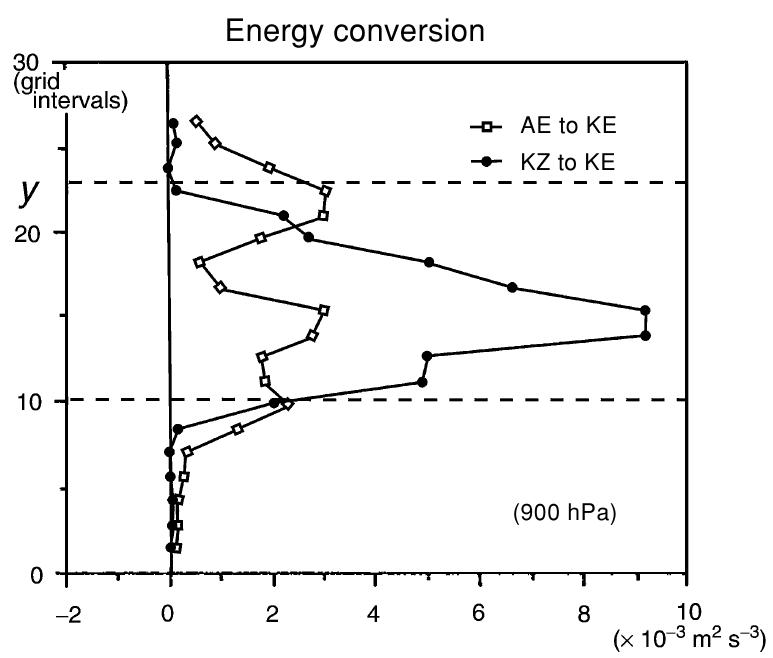
\includegraphics[width=0.5\linewidth]{{./chapters/figures_misc/barotropic_nagata1993}.jpeg}
  \caption{Бароклинная и баротропная конверсия энергии на уровне $900\hpa$ \citep{Nagata1993}.}
  \label{fig:barotropic_nagata1993}
\end{figure}

Согласно \citep{Holton2004}, баротропная неустойчивость --- это волновая неустойчивость, связанная с горизонтальным сдвигом ветра в струйном потоке. Источник роста баротропных возмущений --- кинетической энергии среднего потока.

Подробное исследование полярных мезоциклонов с точки зрения баротропной неустойчивости было проведено, например, для района конвергенции полярной воздушной массы над Японским морем \citep{Nagata1993}. В указанной работе автор отмечает, что в зоне шириной всего несколько десятков километров наблюдаются максимумы завихренности. Для их исследования он применил численную атмосферную модель, которая воспроизвела волны в поле потенциального вихря, которые постепенно обострялись и приобретали вид полярных депрессий с аномалией давления $2$--$4\hpa$. Вихри имели спиралевидную структуру с теплым ядром в центре.

Для подтверждения гипотезы о баротропности наблюдаемых процессов Нагата сопоставляет бароклинный и баротропный источники энергии в полосе вблизи вихря. Пусть $u'$ и $v'$ --- отклонения компонент скорости от среднего потока, то для кинетической энергии формула выглядит следующим образом:
\begin{equation}
K_E = \overline{\frac{1}{2}\left(u'^2 + v'^2\right)}
\end{equation}
Баротропный и бароклинный вклады в трансформацию энергии вычисляются по выражениям
\begin{equation}
C(K_M,K_E)=-\overline{u'v'}\frac{d\overline{u}}{y}
\end{equation}
и
\begin{equation}
C(A_E,K_E)=-\overline{\omega'\alpha'},
\end{equation}
где $K_M$, $K_E$ и $A_E$ --- средняя кинетическая энергия, кинетическая энергия возмущений и доступная потенциальная энергия возмущений соответственно, $\omega'$ --- отклонения вертикальной скорости, $\alpha'$ --- отклонения удельного объема, горизонтальная черта означает осреднение по области.

На рис. \ref{fig:barotropic_nagata1993} представлено распределение интенсивности трансформации энергии по горизонтали. Сравнивая с профилем горизонтального сдвига ветра и профилем кинетической энергии, автор делает вывод, что основным источником вихревых движений является именно сдвиг ветра, чей максимум совпадает с максимумом кинетической энергии. Вклад бароклинной компоненты, как видно из рисунка, по крайней мере в два раза меньше.

Роли баротропных волн в полярном циклогенезе были посвящены и другие работы, объектом которых являлись мезоциклоны в Северной Атлантике и в Беринговом море. К примеру, Дункан, оценивая механизмы развития трех полярных мезоциклонов \citep{RT2003}, заключил, что роль баротропных процессов незначительна. Хотя большинство исследований основывались на структуре полярного струйного течения, Рид \citep{ReedDuncan1987} отмечал, что формирование достаточно резких сдвигов ветра над океанами зимой для развития мезомасштабных вихрей маловероятно.

Итак, атмосферные баротропные волны сами значимы в аспекте образования полярных мезоциклонов по сравнению с бароклинной и термической неустойчивостью (см. следующий раздел). Тем не менее, баротропная неустойчивость иногда может действовать вместе с другими механизмами и даже выступать как триггерный процесс.

\section{Термическая неустойчивость}
\subsection{Условная неустойчивость второго рода}
\subsubsection{Понятие условной неустойчивости}
Динамическая неустойчивость в атмосфере Земли часто связана с неустойчивостью частицы или слоя, то есть определяющее значение имеет сила плавучести. Одним из механизмов, предложенных для объяснения полярных мезоциклонов, является условная неустойчивость второго рода (conditional instability of second kind, CISK). 

Условная неустойчивость – понятие, близкое к статической неустойчивости, и также базируется на разности плотности между частицей воздуха и окружающей атмосферы. Основное отличие состоит в том, что при определении условной неустойчивости принимается во внимание насыщенность воздуха, в то время как статическая устойчивость предполагает влажность равную либо $0$, либо $100\%$. Критерием условной неустойчивости является вертикальный градиент псевдопотенциальной температуры (эквивалентной потенциальной температуры при насыщении).

Помимо обычного взгляда на условную неустойчивость в терминах градиентов потенциальной температуры, в контексте данной работы необходимо привести 'энергетическое' определение, в котором используется понятие конвективной доступной потенциальной энергии (convective available potential energy, CAPE):
\begin{equation}
CAPE_i = \int_{z_{i}}^{z{LNB}} g\frac{T-\overline{T}}{T}dz,
\end{equation}
где $CAPE_i$ --- конвективная доступная потенциальная энергия частицы, $z_{i}$ --- высота, на которой находится частица, $z_{LNB}$ --- уровень нейтральной плавучести, $T$ --- температура частицы, $\overline{T}$ --- температура окружающего воздуха. То есть частица воздуха обладает условной неустойчивостью при положительной энергии плавучести ($CAPE_i>0$). Точнее, для ненасыщенного воздуха устойчивость может быть в двух вариантах: 1) $CAPE=0$: устойчивость для всех вертикальных движений, 2) $CAPE>0$: неустойчивость для вертикальных движений конечной амплитуды, которая, в свою очередь, может быть двух типов: $CAPE>CIN$ и $CIN>CAPE$ \citep{Lin2007}.

Минусом метода частицы является неспособность описать неустойчивости, связанные с горизонтальным градиентом температуры (бароклинную и баротропную неустойчивость). Кроме того, в ней не учитываются некоторые процессы, уменьшающие силу плавучести, а именно эффект вовлечения, влияние конденсированной влаги на плотность воздуха и компенсирующие движения окружающего воздуха в ответ на формирование облаков.

\subsubsection{Условная неустойчивость второго рода}
Некоторые из указанных процессов включены в концепцию условной неустойчивости второго рода (CISK). Она была впервые применена Чарни и Элиассеном в работе по тропическому циклогенезу и подразумевает следующее:
\begin{sqlist} 
\item Выделение скрытого тепла при конвекции приводит к образованию циклонического возмущения в нижней тропосфере.
\item Циклоническая аномалия создает условия для конвергенции влаги благодаря трению в пограничном слое (Экмановская подкачка).
\item Конвергенция потоков способствует подъему условно неустойчивого воздуха на уровень свободной конвекции и выделению скрытого тепла конденсации.
\end{sqlist}
Принципиальная схема условной неустойчивости второго рода показана на рис. \ref{fig:cisk_rt2003}.

Роль глубокой конвекции в эволюции полярных мезоциклонов подчеркивалась в работах Расмуссена и Окланда \citep{RT2003}. Они справедливо заявляли, что устойчивость арктических воздушных масс резко уменьшается при холодных вторжениях на поверхность океана.

\begin{figure}[!ht]
	\centering
	\begin{subfigure}[t]{0.4\textwidth}
		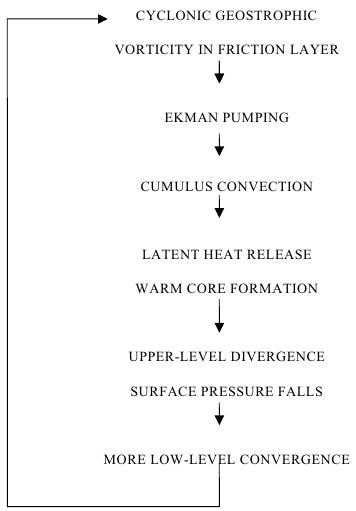
\includegraphics[width=\linewidth]{{./chapters/figures_misc/cisk_rt2003}.jpeg}
		\caption{ }
		\label{fig:cisk_rt2003}
	\end{subfigure}
	\hfill
	\begin{subfigure}[t]{0.4\textwidth}
		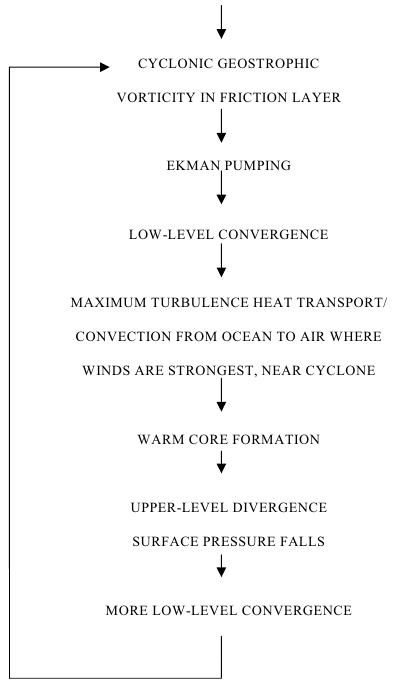
\includegraphics[width=\linewidth]{{./chapters/figures_misc/wishe_rt2003}.jpeg}
		\caption{ }
		\label{fig:wishe_rt2003}
	\end{subfigure}
	\caption{Принципиальная схема CISK (a) и WISHE (b) \citep{RT2003}.}
\end{figure}

Теоретические исследования были продолжены с применением сначала аналитической модели \citep{SardieWarner1983} в двумерных квазигеострофических уравнениях, учитывающих диабатические источники тепла. После сравнения с данными наблюдений семи случаев было показано, что эффектов CISK недостаточно для описания скорости роста ни атлантических мезоциклонов, ни тихоокеанских. С другой стороны, недостаточно и влияние только 'сухой' бароклинности. Однако при суперпозиции условной неустойчивости и бароклинности результаты оказываются близкими к реальности. При этом наилучшее совпадение с наблюдениями показывают те результаты, включающие эффекты CISK во влажной бароклинной атмосфере. Этот в некоторой степени очевидный факт объясняется тем, что при наложении бароклинности и конвективной неустойчивости тепло выделяется как в кучевой, так и в слоистой облачности. Другими словами, в нижних слоях атмосферы существует источник бароклинной доступной потенциальной энергии, который дополняется на высотах источником энергии фазовых переходов. Выводы, сделанные в аналитическом подходе к проблеме, подтверждаются ре-зультатами численного моделирования \citep{SardieWarner1983}.

Одной из новейших работ, посвященных анализу динамики полярных мезоциклонов с точки зрения конвективной доступной потенциальной энергии является статья \citep{LindersSaetra2012}. В ней с помощью набора данных, полученных в ходе эксперимента в Северном море, доказывается, что, во-первых, условная неустойчивость фактически отсутствует, а во-вторых, опять же в контексте полярных мезоциклонов величина CAPE сравнима с потоком тепла с поверхности океана за ограниченное время и, таким образом, не представляет важного компонента бюджета энергии мезоциклона.

\subsection{WISHE}
На замену теории неустойчивости второго рода пришла теория интенсификации циклона под действием потоков тепла с поверхности \citep{EmanuelRotunno1989}. В данной концепции предполагается, что атмосфера нейтрально устойчива по отношению к влажной конвекции. Это верно для районов формирования тропических циклонов, для которых и разрабатывалась данная теория. Влажная конвекция перемешивает нижние слои тропосферы, но не приводит к образованию значительной температурной аномалии в случае отсутствия источника явного или скрытого тепла с поверхности. Потоки тепла с поверхности зависят от скорости ветра и, следовательно, определяются интенсивностью вращения вихря. Другими словами, имеется четкая обратная связь между интенсивностью мезоциклона и нагревом от подстилающей поверхности \ref{fig:wishe_rt2003}.

Можно заметить, что отличие теории WISHE от приведенной в предыдущем разделе состоит в том, каким образом связана конвекция с интенсивностью циклона. То есть в случае WISHE максимальная неустойчивость наблюдается в районах с максимальным ветром и не включает совместного влияния конвергенции под действием силы трения.

По современным представлениям, WISHE остается одной из наиболее продвинутых концепций в теории генезиса как тропических \citep{CraigGray1996}, так и полярных вихрей \citep{EmanuelRotunno1989}. Тем не менее, этот механизм имеет свои недостатки, в частности, предположение о градиентном балансе в пограничном слое, а также об осесимметричности вихря. И теория CISK, и теория WISHE не описывают процесс зарождения возмущения. Например, Эмануэль citep{EmanuelRotunno1989} отмечает, что для поддержания WISHE атмосферный вихрь уже должен существовать в виде возмущения конечной амплитуды.

\section{Влияние подстилающей поверхности на развитие полярных мезоциклонов}
В атмосфере полярных регионов как бароклинные, так и конвективные процессы часто наблюдаются вблизи границы льда или снежного покрова. Они связаны с температурным градиентом между охлажденной поверхностью льда и относительно теплой поверхностью воды, достигающим несколько десятков градусов. Также возникают значительные контрасты альбедо и шероховатости. Из-за этого энергетический бюджет пограничного слоя над открытой водой и над поверхностью льда существенно отличается.

\begin{figure}
  \centering
  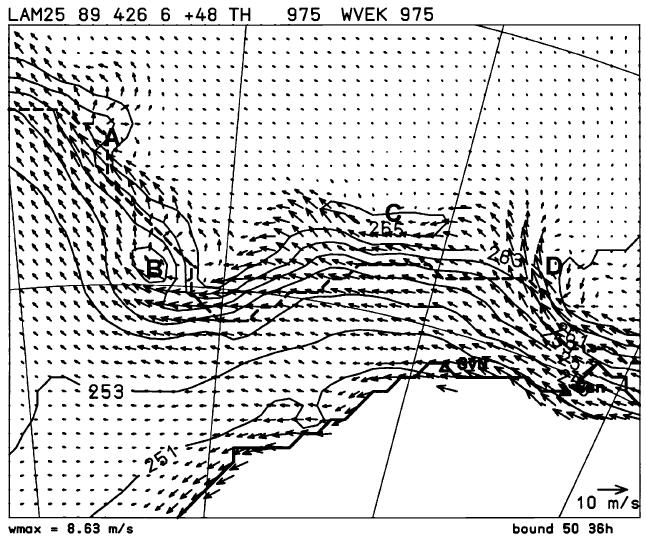
\includegraphics[width=0.5\linewidth]{{./chapters/figures_misc/heinemann1996a}.jpeg}
  \caption{Потенциальная температура (сплошные линии через $2\K$) и вектора скорости на уровне $975\hpa$. Буквами обозначены отдельные мезоциклоны \citep{RT2003}.}
  \label{fig:heinemann}
\end{figure}

Удобная для генерации мезоциклонов резкая бароклинная зона, или фронт пограничного слоя (ФПС) часто формируется, когда воздушный поток направлен почти параллельно границе ледового покрова. Процессы фронтогенеза ведут к образованию облачных валиков, что четко видно на спутниковых снимках. В результате отклонений поля ветра от среднего полярный может происходить адвекция ФПС. Тогда создаются благоприятные условия для формирования вихря. Полярные мезоциклоны такого типа классифицируются как системы на Арктическом/Антарктическом фронте и питаются за счет бароклинной неустойчивости и мощных потоков тепла с поверхности воды.

В данном разделе коротко обсуждаются результаты исследований за последние два десятилетия, в которых предметом являлось взаимодействие поверхности океана, частично покрытой льдом, и динамики мезоциклона, зарождающегося или переносящегося над этой областью.

Одним из первых данной проблемой занялся Хайнеманн \citep{Heinemann1997}, используя модель NORLAM, проводивший идеализированные эксперименты для конкретной территории, а именно моря Уэделла. Изначально однородные по горизонтали метеополя были деформированы в результате поверхностного форсинга, что выразилось, в частности в падении давления в поясе вдоль границы льда. Это сопровождалось резким усилением скорости ветра, образования зоны конвергенции над водой и температурного градиента около $5\K$ на $50\km$.

При этом геострофическая компонента скорости ветра была направлена квазипараллельно фронту, агеострофическая --- со льда на воду. Граница льда была построена по данным наблюдений и в ледовом покрове существовали неоднородности в виде заливов и выступов. Именно в этих областях, как и ожидалось, возникали условия для генерации завихренности \ref{fig:heinemann}. Однако, как доказывает автор, возникшая серия вихрей состояла из мезоциклонов, слабо развитых по высоте и не прослеживающихся на уровне $700\hpa$ даже через трое суток моделирования.

Похожее исследование, основанное на данных натурных измерений, было проведено и для Гудзонова залива \citep{AlbrightEtAl1995}. В одном из экспериментов температура поверхности океана (ТПО) была увеличена на $8\K$, что привело к серьезному усилению полярного вихря до скоростей, превышающих ураганные значения. Кроме влияния ТПО, авторы обнаружили сильную зависимость динамики мезоциклона от формы границы льда: при замене реальной границы на идеально прямую меридионально расположенную, вихрь существенно поменял свою траекторию и уменьшил скорость своего роста.

Что касается температуры поверхности, то ее влияние на эволюцию мезоциклона было проанализировано в работе \citep{AdakudluBarstad2011}. В ней показано, что аномалия давления в центре полярной депрессии росла в зависимости от вариаций ТПО со скоростью около $2\hpa\K^{-1}$.

\begin{figure}
  \centering
  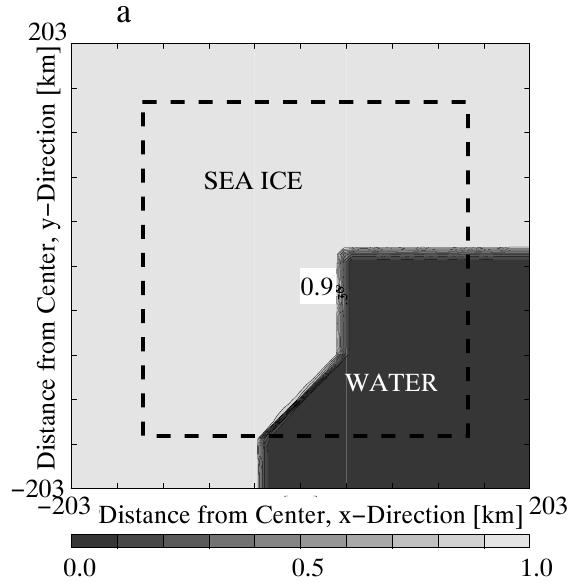
\includegraphics[width=0.5\linewidth]{{./chapters/figures_misc/ds2005}.jpeg}
  \caption{Распределение льда и воды в экспериментах \citep{DiererSchluenzen2005}.}
  \label{fig:ds2005}
\end{figure}

Более идеализированное исследование \citep{DiererSchluenzen2005} было призвано оценить взаимодействие между мезоциклоном и  параметрами ледяного покрова, включая толщину льда, соотношение льда и воды на единице площади и др. Форма границы льда была одной и той же для всех экспериментов и имела вид угловой ступеньки в юго-восточной части области интегрирования \ref{fig:ds2005}. В отличие от многих других работ, здесь явно учитывались и процессы в океане, а наличие морского течения.
 
Наиболее важным параметром оказалось распределение льда, которое определяет градиент температуры между поверхностью и приземным слоем воздуха. Кроме того, наименьший средний поток тепла наблюдался при смещенном треке мезоциклона. Морское течение и толщина льда почти не влияют на тенденцию давления. Наибольшие отличия тенденции давления по сравнению с контрольным экспериментом наблюдаются в эксперименте с однородным льдом и со смещенным треком. В первом случае мезоциклон сам 'сдвигает' лед, и в результате в районе неоднородной концентрации льда развивается бароклинный слой.

Говоря о результатах указанной работы, отметим, что параметры, влияющие на вариации давления и скорости ветра, проявляются и в значимых изменениях потоков тепла с поверхности. Влиянием мелкомасштабных изменений потоков (из-за толщины льда или морских течений) можно пренебречь. Менее плотный ледовый покров (с присутствием пятен открытой воды) и большие скорости ветра являются благоприятными условиями для дальнейшего разрежения льда и возникновению положительной обратной связи.


\begin{thebibliography}{12}
 \bibitem{ER89}
Emanuel KA, Rotunno R. 1989. Polar lows as Arctic hurricanes. \textit{Tellus} \textbf{41A:} 1-17.
\end{thebibliography}

\end{document}